\documentclass[preprint,12pt]{elsarticle}

\usepackage{graphics}
\usepackage{float}
\usepackage{epsfig}
\usepackage{dcolumn}
\usepackage[implicit=false]{hyperref}
\usepackage{amsthm}
\usepackage{algorithmicx}
\usepackage{algpseudocode}
\usepackage{latexsym}
\usepackage{algorithm}
\usepackage{caption}
\usepackage{multirow}
\usepackage{stmaryrd}
\usepackage{amssymb}
\usepackage{latexsym}
\usepackage{color}
\usepackage{rotating}
\usepackage{tabularx}


\journal{Lorentz Center Meeting}


\newcommand{\mi}[1]{\ensuremath{\mathit{#1}}}
\theoremstyle{definition}
\newtheorem{definition}{Definition}
\newcommand{\todo}[1]{\textcolor{red}{#1}}


\begin{document}
\begin{frontmatter}

\title{Opportunistic sensing to improve bike road infrastructure}

\author{RWS group}
%\ead{e.kaldeli@rug.nl}
%\address{University of Groningen}


%% \title{Title\tnoteref{label1}}
%% \tnotetext[label1]{}
%% \author{Name\corref{cor1}\fnref{label2}}
%% \ead{email address}
%% \ead[url]{home page}
%% \fntext[label2]{}
%% \cortext[cor1]{}
%% \address{Address\fnref{label3}}
%% \fntext[label3]{}


%% use optional labels to link authors explicitly to addresses:
%% \author[label1,label2]{<author name>}
%% \address[label1]{<address>}
%% \address[label2]{<address>}





%\begin{abstract}
%An executive summary should go here.
%\end{abstract}



%\begin{keyword}
%\end{keyword}

\end{frontmatter}


\section{Context}
Rijkswaterstaat from the Ministry of Infrastructure and the
Environment is interested to investigate how citizens, for instance
while cycling, can provide information about the infrastructure they
are using without significant involvement and without increasing the
risk of accidents. Given the current context of the Netherlands that
indicates that 4 million citizens use smartphones while traveling and
that 50\% of Dutch bikers read social media messages while biking, one
may take advantage of the sensing capabilities of smartphones while
people are active on their bikes. The challenges are, on the one hand, to understand
what is possible to infer about the infrastructure from using the
sensing capabilities of a smartphone and, on the other hand, to design
an app which is easy to use, doesn't endanger the user while biking,
is appealing and engaging to employ and guarantees sufficient privacy
to the end-user. 


\section{State of the art}

The pervasiveness of smart devices has open a number of unprecedented
opportunities for what falls under the name of {\em
  crowdsensing}~\cite{gan:mob11}. Modern smartphones have a wide
pletora of sensing interfaces which make interaction with the physical
environment easy and information rich, for instance, a modern iPhone
has: three-axis gyro, accelerometer, magnetometer, GPS, proximity
sensor, ambient light sensor, two high resolution cameras, a
microphone and high-frequency networking interfaces. These have been
exploited for a number of pattern recognition taks,
e.g.~\cite{fuj:iph10}. The specific issue of identifying the quality
of bike paths using dedicated sensors on board of bicycles has been
proposed in~\cite{eis:bik07} while possible social interactions of
bikers have been investigated
in~\cite{red:bik10}. In~\cite{eri:pot08}, the authors consider vehicle
onboard sensing to measure road quality with dedicated solutions.



\section{Problem definition}

\subsection{Infrastructure quality}

One has to first define what are relevant parameters that influence
the infrastructure quality, in our case, bike paths. The relevant
elements appear to be, in order of relevance,
\begin{enumerate}
\item presence of major potholes or other large size obstacles
\item coarseness/smoothness of the biking surface (in relation to the
  material used to create the infrastructure and its age)
\item weather conditions (wetness, ice, snow, in particular)
\item path traffic 
\item neighboring/interfering car traffic
\item quality of air (e.g., CO2 levels)
\item illumination
\end{enumerate}


\subsection{Sensing}

To measure the quality of the infrastructure just listed, we plan to
consider using a smartphone. Precise design choices can be defined
only after experimentation (see Pilot project section). We consider
the following relevant assumptions/choices.
\begin{description}
\item[Position of the phone.] Placing the phone on the frame of the
  bike or handle appears to make the sensing easier and more
  consistent across cyclist, though might be harder for the user to
  accept and will require extra equipment.
\item[Accelerometer.] This sensor is essential, but might not provide
  enough information.
\item[GPS.] Necessary for path tracking, reporting problems on
  specific location, report average speeds on given tracks.
\item[Gyroscope.] Very useful, especially if the phone is on the
  person and not on the bike. It may also help detect hazardous
  situations, such as the fall of the biker.
\item[Light sensor.] Might help in darkness conditions, if the phone
  is on the bike.
\item[Magnetometer.] Might help to detect the amount of surrounding
  cars.
\item[Camera.] Very useful, but putting too much computational and
  battery stress on the phone, therefore ignored in the following.
\end{description}


\subsection{Distribution architecture: data management and privacy}

There is an important issue on where the data processing occurs and
where raw and inferred data is stored. Another related relevant
problem is on when is data transferred from the mobile devices to the
data aggregation points. We foresee a solution in which raw data is
processed locally on the smartphone, inferred data is transmitted to
the RWS servers when the user docks in his base station (e.g., work or
home pc), unless a dangerous situation requires immediate data transmission
(major infrastructure problem or accident to the cyclist). Also the
storage of the data implies important privacy concerns. The sensed
data includes highly sensitive information on the location and
behaviors of the end user. Storing on the mobile phone is neither
feasible nor useful. Storing centrally anonymously seems important,
though not giving sufficient privacy guarantees. On the other hand,
having user profiles related to sensed data, would highly increase the
quality of the acquired data.

\begin{figure}[ht]
\begin{center}
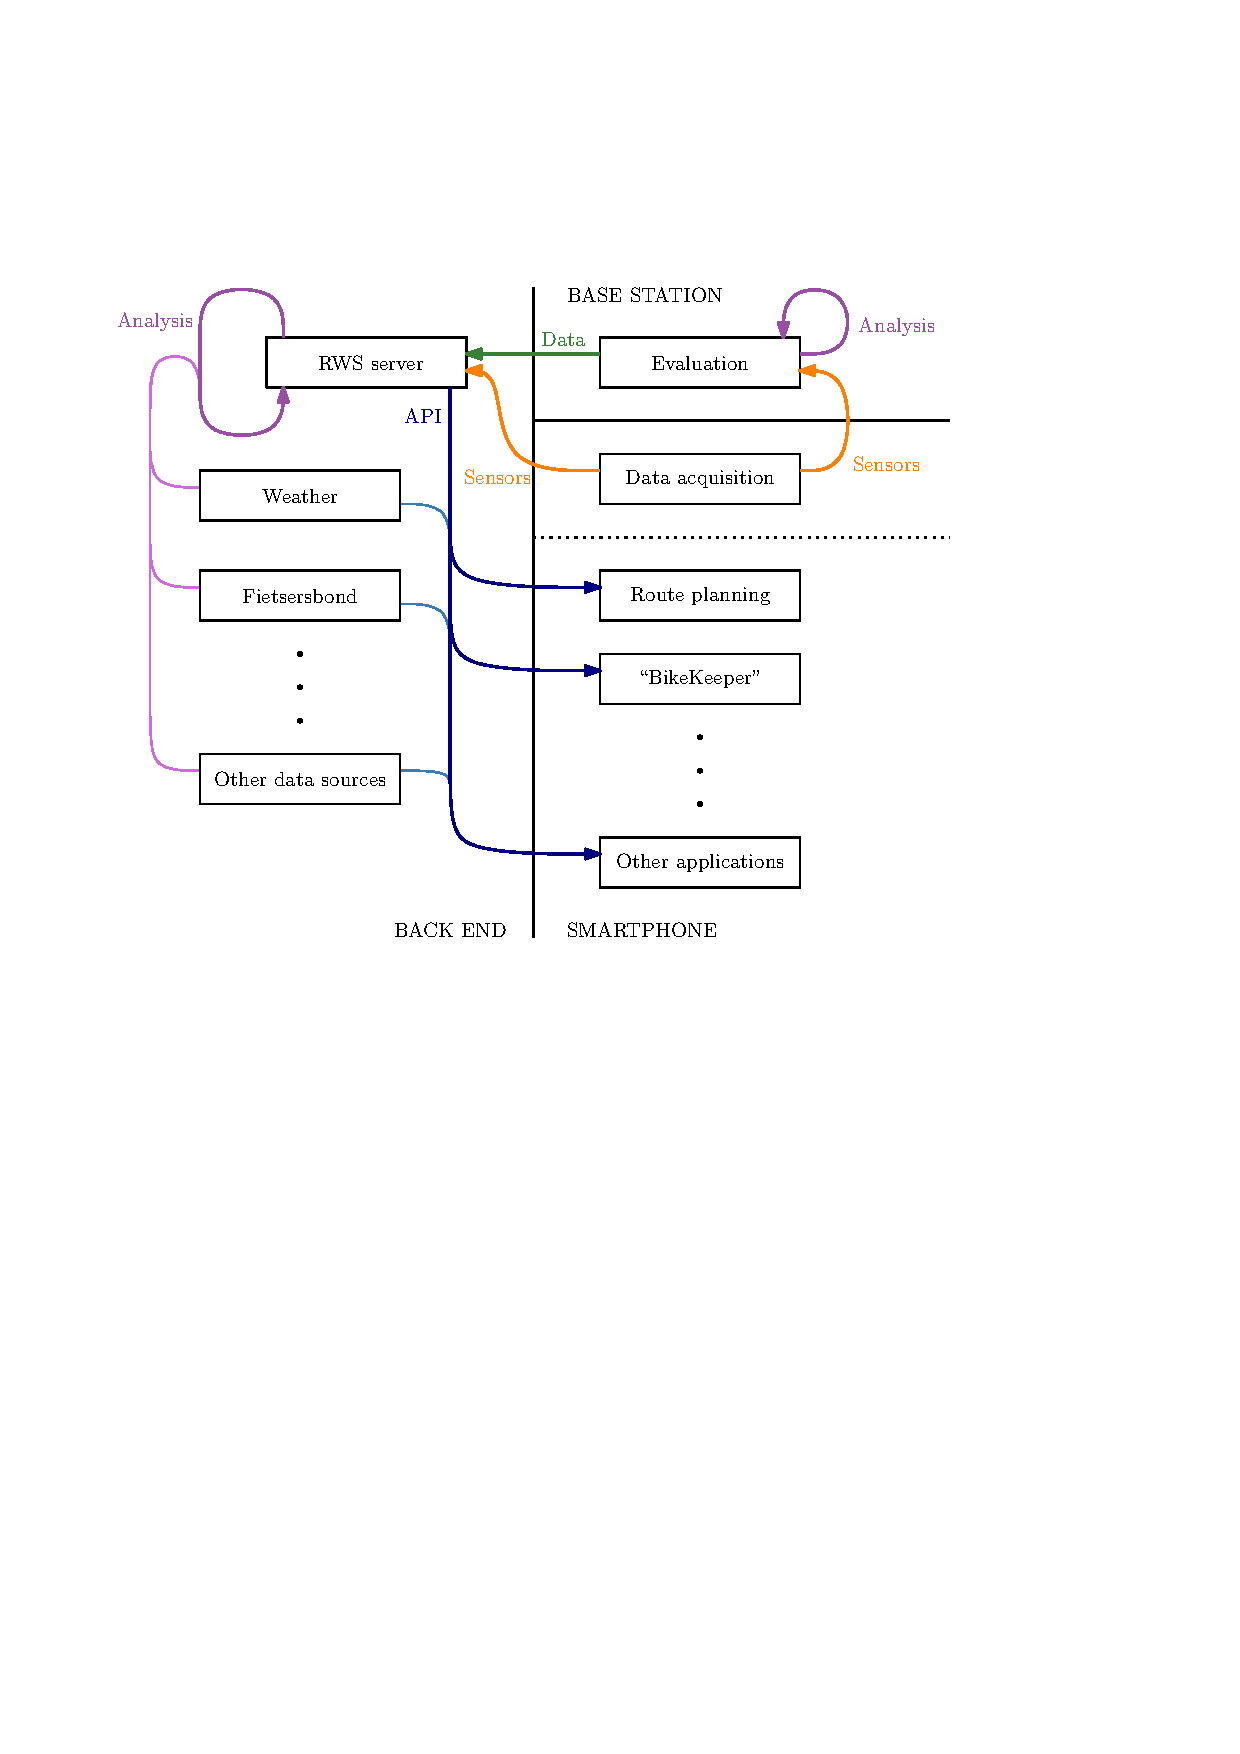
\includegraphics[width=100mm]{figures/systemoverview}
\caption{Architectural overview.\label{fig:sys}}
\end{center}
\end{figure}

A possible high-level architectural overview of the system is
presented in Figure~\ref{fig:sys}. The smartphone (on the
bottom-right) is responsible for the opportunistic sensing and user
interaction, thus acquiring the raw data. The data is then processed
on a base station (on the top-right), possibly in the control of the
end user. Raw data is transformed into meaningful infrastructure
events. The smartphone also has extra components which create added
value for the end user and can help foster his adoption  and usage of
the app, namely, a routeplanner, a biometric ``BikeKeeper'' component
for the tracking of physical activities, and so on. The events
acquired by the individuals are then aggregated on the back end
servers (on the left of the figure). The event and possibly raw sensor
data are also correlated with relevant external information, such as
that on the weather, from other sources monitoring the quality of the
roads, such as Fietsersbond, etc.



\subsection{User interaction}

The user should minimize the interaction with the app. If the app
provides extra features (e.g., traffic information, turn by turn
routing, biometrics), these should be presented to the user without
distracting him/her from the driving. The opportunistic sensing should
be done in the background and user confirmation should occur as an ex
post notification. For instance, when docking the user is prompted to
confirm that a strong acceleration was related to a major pothole in
the pavement. 


\subsection{Incentive scheme}

One has to design an effective incentive scheme for the end user. Some
will be willing to help the community independently of any personal
advantage. We fear that though these kind of users will be a
minority. Other incentives might come from the certainty that
reporting infrastructural problems will improve a route that the user
frequently follows. More short term high reward incentives, might come
from having a free navigation and traffic information system be given
``for free'' with the infrastructure monitoring app. A quantitative
study of what works is necessary to establish an effective marketing
strategy for the app.


\section{Scenarios of application}

\subsection{Stakeholders}

\subsection{Scenario - The bike enthusiast}

The weather is nice outside; Frank decides to go out for a ride. 
He slides his smartphone in the holder that is attached to his steer. He opens the RWS app and presses “Start”. The app starts to record the GPS and accelerometer data. 
While cycling through nice scenery, Frank sees a big gap in the road. He thinks that this could be a potentially hazardous situation. He presses the “take photo” button to directly take a shot of the gap, and decides to share the photo with the RWS. The photo includes GPS data, so the road maintenance department can directly judge if they should repair it. 
He decides to go on and when he arrives at home he presses the “Stop” button, to stop the recording. When he is connected to Wi-Fi, the app asks to upload his data.
When he opens the RWS web-interface on his PC, the recorded journey is shown on a map. There is an overlay with indications of bad stretches of road surface, which are based on the accelerometer data. If an indication is right, he can click on a tick box to verify. When he is finished he can share this information with RWS.  


\subsection{Scenario - The commuter}

Vincent commutes every day to his work. Since he lives just outside the city it takes him 20 minutes to travel to his work. He really likes the idea that he can personally help improving the roads and bike lanes he is using everyday.
When leaving his house he slides his smartphone in the holder and opens the app. He presses the “Start” button to start recording.
When he arrives at work he presses the “Stop” button. When he enters the building his smartphone automatically connects to the Wi-Fi and the app asks to upload the data, which he allows. Vincent doesn’t have any time to verify the potential bad stretches of road. Nonetheless the information is useful.


\subsection{Scenario - OV-fiets}

Marja decides to go to Zandvoort for a day. When she arrives she rents an OV-fiets at the train station.
The OV-fiets contains a recording device with GPS and an accelerometer. 
The device notices it when Marja’s rented bike leaves the bicycle storage and starts recording automatically. While cycling around Zandvoort she stops once in a while for a break. The device detects this and pauses the recording. It starts again when the bicycle is used.
When Marja returns her bike at an OV-fiets location the device stops recording and uploads the data automatically. 




\section{Pilot project to check feasibility}

To come to a first design of a solution, we propose to run a
pilot project to acquire evidence of what kind of sensing provides
readings that correlate to infrastructure quality. The experiment will
be designed in the following way.

\begin{description}
\item[Ground truth construction]\mbox{}\\[-2ex]
\noindent
  \begin{enumerate}
  \item RWS will provide a classification of
    infrastructure based on its known construction and aging
    qualities. 
  \item RWS will also provide a classification of faults that can be
    present in the infrastructure (e.g., pothole classification)
  \item RWS will provide geographical indications of where an instance
    of each of the types of roads and faults are present in the
    infrastructure. These should be defined as stretches of about
    50-100 meters. These should be geographically close to each 
    \item The research team will videorecord cyclist pedaling on such
      identified stretches.
    \item The research team will manually annotate the videos
      indicating quality properties of the infrastructure. The
      annotations are then related to geographical location with an
      accuracy of at least 1 meter.
\end{enumerate}

\item[Sensor readings]\mbox{}\\
%  \begin{enumerate}
%    \item 
      The research team will perform sensor readings utilizing all
      sensors of a smartphone by running over the identified road
      stretches. For each stretch, at least 5 different configurations
      are used. Each configuration entails a unique type of bicycle
      and a unique user. Each test is repeated at least 6 times. 3
      times with the phone attached in solid to the bike and 3
      times with the phone on the user (pants, jacket, backpack).
%  \end{enumerate}

\item[Data Analysis]\mbox{}\\
%  \begin{enumerate}
%   \item 
      The research team will then analyse the acquired sensor data and
      compared it with the ground truth in order to find correlations
      between sensor readings and infrastructure qualities. 
%  \end{enumerate}
\end{description} 

The end results of the pilot is to come to a preliminary conclusion of
what are the possible sensor readings and bike-user configurations
that allow an assessment of the infrastructure quality. It also allows
to understand the volume and velocity of sensor produced data and
types of data analysis necessary to transform raw data into
events. This will allow to make a design that answers the first
challenge of the project: that is opportunistic sensing. The next
problem to then be addressed is the distributed architecture. Finally,
having solved the data management issues, one can then move on to the
second research question: user engagement and safety.






\section{The way ahead}

Give us a lot of money and we can solve anything.



\bibliographystyle{apalike}
\bibliography{rws}
\end{document}






